\clearpage
\slidetitle{Un algorithme de séparation}

\begin{slide}

	\begin{itemize}

		\item Sélection de chaque pixel et de ses pixels adjacents et stockage des groupes temporaires ainsi formés dans une liste $T$.
		\item Initialisation d'une liste (vide) de caractères $C$ (groupes de pixels).
		\item Pour chaque groupe temporaire $a \in T$, et pour chaque caractère $b \in C$, $a$ prend la valeur $a\cup b$ si $a\cap b \neq \emptyset$ et on enlève $b$ de $C$. 
		\item À la fin de la boucle qui parcourt $T$, on ajoute $a$ à $C$, même s'il n'a pas été modifié.

	\end{itemize}

	\begin{figure}[h!]
		\centering
		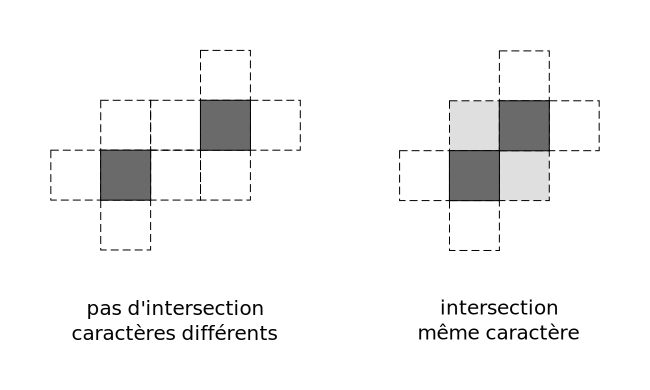
\includegraphics[width=0.8\linewidth]{schemas/algo_sep2.pdf}
	\end{figure}


\end{slide}